
In the semiconductor sensors a charged particle creates electron-hole pairs which drift under the influence of an electric field to the read-out electrodes. If all charge carriers are collected by a single strip/pixel, the position resolution depends only on the distance between strips/pixels, i.e. on pitch size. If the lateral broadening of the charge is compared with the strip/pixel pitch, the part of the charge may be collected at a neighboring strip/pixel. This effect, called charge sharing, can improve the accuracy of the position resolution. The charge sharing could be achieved by using the magnetic field, by tilting the sensor or increasing the lateral size of the charge distribution during the drift.

The charge carriers drift along the lines of electric field. In order to spread the charge in the lateral direction, the electric field should be modified. To manipulate the electric field, deep implants are used. The p+ implants in a p-bulk sensor are conceived by incorporation of Boron atoms, and  create a repulsive area for electrons. When the electron cloud meets a p+ implant on the drifting way, the former splits into two halves fig.1 (left). Applying it layer-wise gives the charge sharing between three strips/pixels fig.1 (right).  The charge cloud is split 50/50 on every layer, which gives a binomial distribution of the charge.

\begin{figure}[h]
\center{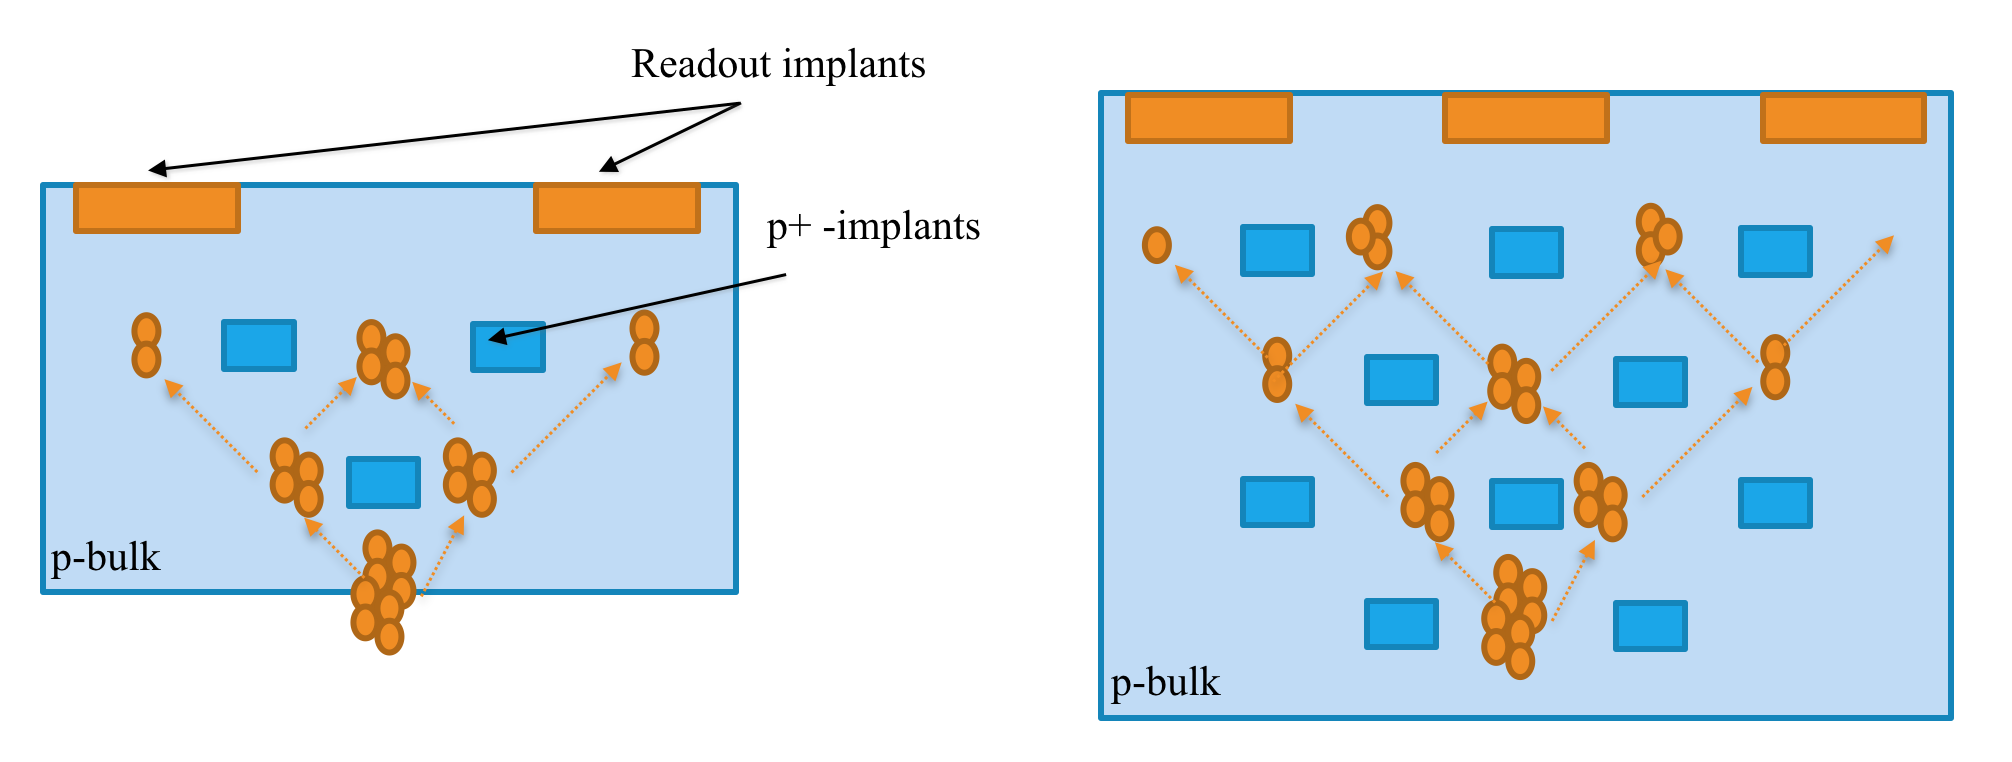
\includegraphics[width=12cm]{/Users/tweety/Documents/PhD/TIPP/TIPP17/pictures/binomial.png}}

Fig. 1. The example of the 50/50 charge sharing in the ELAD sensor. 
\end{figure}

The binomial charge distribution gives a cluster size of 3 that is not optimal. The neighboring strips may collect not enough charge to pass the sensor's threshold. More efficient charge sharing is achieved at a value of cluster size of 2. In order to obtain this value of the cluster size, it is necessary to change the position of the implants. Usage of p+ deep implants leads to the increase of the value of the doping concentration in the sensor. This causes to increasing of the value of $N_{eff}$. The high value of $N_{eff}$ induces the increase of the depletion voltage. 

\begin{equation}
N_{eff}=N_{D}-N_{A}
\end{equation}

\begin{equation}
V_{depl}=\frac{q_0 D^2 |N_{eff}|}{2 \epsilon_r \epsilon_0 }
\end{equation}

To control the value of $N_{eff}$ deep p+ and n+ implants are used. The implants are located between 2 strips/pixels, which gives a cluster size of 2. The n+ implants are placed between two p+ implants. If the doping concentrations of p+ and n+ implants are carefully balanced, the value of $N_{eff}$ and, correspondingly, $V_{depl}$ remains not to high. The number of implant layers should be as small as possible due to the difficult production process. 
